\documentclass[12pt]{article}
\usepackage{graphicx}
\graphicspath{ {./images/} }
\usepackage[utf8]{inputenc}
\usepackage{amsthm,xpatch}
\usepackage{amsmath}
\usepackage{tikz} 
\usepackage{geometry}
\usepackage{amssymb}
\usepackage{enumerate}
\usepackage{float}
\usetikzlibrary{arrows, automata, calc, positioning}
\geometry{margin=2cm}

\title{MLCS - Homework 2}
\author{Michele Conti \\ \texttt{1599133}}
\date{}


\theoremstyle{definition}
\newtheorem{exerciseinner}{Exercise}
\newenvironment{exercise}[1]{%
	\renewcommand\theexerciseinner{#1}%
	\exerciseinner
}{\endexerciseinner}

\renewcommand*{\proofname}{Solution}

\makeatletter
\newcounter{proofpart}
\xpretocmd{\proof}{\setcounter{proofpart}{0}}{}{}
\newcommand{\proofpart}[1]{%
	\par
	\addvspace{\medskipamount}%
	\stepcounter{proofpart}%
	\noindent\emph{{Part \theproofpart: #1}}\par\nobreak\smallskip
	\@afterheading
}
\makeatother

\begin{document}
\maketitle

\section{EF-games and (non)-expressibility}

\begin{exercise}{1.5}
	Consider the following two structures (for the language of graphs):
	\begin{enumerate}[\quad{(}1{)}]
		\item $\mathfrak{G}_1$ is a cycle of length $4n$;
		\item $\mathfrak{G}_2$ consists of two disjoint cycles of length $2n$.
	\end{enumerate}
	Analyze the EF games on these structures for $n = 1, 2$ and write a sentence of minimal quantifier rank distinguishing the two structures for $n = 1, 2$.
	
	BONUS: Formulate a generalization of your observation and prove that the Connectivity query is not expressible in the language of graphs over finite graphs, using EF-games.
\end{exercise}
\begin{proof}
	Let's discuss every point separately.
	\proofpart{$n = 1$.}
	In this case, $\mathfrak{G}_1$ is a cycle of length $4$:
	\begin{figure}[H]
	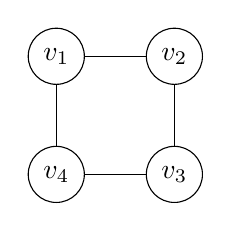
\begin{tikzpicture}[node distance={15mm}, main/.style = {draw, circle}]
		\node[main] (1) {$v_1$};
		\node[main] (2) [right of=1] {$v_2$};
		\node[main] (3) [below of=2] {$v_3$};
		\node[main] (4) [left of=3] {$v_4$};
		\draw (1) -- (2);
		\draw (2) -- (3);
		\draw (3) -- (4);
		\draw (4) -- (1);
	\end{tikzpicture}
	\centering
	\caption{Structure $\mathfrak{G}_1$, consisting of a cycle of length $4$.}
\end{figure}
	\noindent
	While $\mathfrak{G}_2$ is the disjoint structure composed by two cycles of length $2$:
	\begin{figure}[H]
	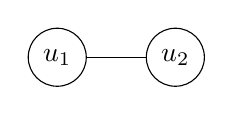
\begin{tikzpicture}[node distance={15mm}, main/.style = {draw, circle}]
		\node[main] (1) {$u_1$};
		\node[main] (2) [right of=1] {$u_2$};
		\draw (1) -- (2);
	\end{tikzpicture}
	\hspace{3cm}
	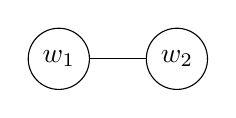
\begin{tikzpicture}[node distance={15mm}, main/.style = {draw, circle}]
		\node[main] (1) {$w_1$};
		\node[main] (2) [right of=1] {$w_2$};
		\draw (1) -- (2);
	\end{tikzpicture}
	\centering
	\caption{Structure $\mathfrak{G}_2$, consisting of two cycles of length $2$.}
\end{figure}
	
	Let's now simulate a match of the EF-games, analyzing each round individually from both Spoiler's and Discriminator's point of view. For each round, we will consider all possible scenarios, in order to completely solve the game. We will adopt the usual EF rules:
	
	\begin{itemize}
		\item Spoiler always starts first.
		\item If a player chooses his node from one of the two structures, the other player must necessarily choose his node from the other structure.
		\item Spoiler always tries to win the game in as few moves as possible, while Discriminator always tries to prolong the game as long as possible.
	\end{itemize}
	
	\noindent\textbf{Round 1}:
	
	During the first round, each player freely chooses a node from one of the structures. There is no special case to mention.
	
	\noindent\textbf{Round 2}:
	
	During the second round, Spoiler can either select a node connected to the first one, or select a node disconnected from the first one. Either way, Discriminator can respond with a similar move, since both structures contain both connected and disconnected nodes (e.g., in $\mathfrak{G}_1$ $v_1$ and $v_2$ are connected, while $v_1$ and $v_3$ are not. As for $\mathfrak{G}_2$, $u_1$ and $u_2$ are connected, while $u_1$ and $w_1$ are not).
	
	\noindent\textbf{Round 3}:
	
	Spoiler chooses two connected nodes in structure $\mathfrak{G}_1$ in the first two rounds, in the third round he chooses a third node connected to either of the previous two. Therefore, Spoiler wins, since there are no 3 connected nodes in structure $\mathfrak{G}_2$.
	
	\noindent\textbf{Conclusion}:
	
	We saw that Discriminator can win all 2-rounds games on these structures, while he has no winning condition on some of the 3-rounds games. Therefore, $\mathfrak{G}_1$ and $\mathfrak{G}_2$ cannot be distinguished by a sentence of a quantifier-rank $2$ or less (i.e., $\mathfrak{G}_1 \equiv_2 \mathfrak{G}_2$), and there is a sentence of quantifier-rank $3$ with which we can distinguish the two structure (i.e., $\mathfrak{G}_1 \not\equiv_3 \mathfrak{G}_2$).
	
	Specifically, the sentence we empirically used during the game is the one expressing the existence of 3 connected nodes. Formally:
	
	\[
	\exists v_1 \exists v_2 \exists v_3 (E(v_1, v_2) \land E(v_2, v_3)),
	\]
	where $E(a, b)$ expresses the existence of an edge between nodes $a$ and $b$.
	
	\proofpart{$n = 2$.}
	For $n = 2$, $\mathfrak{G}_1$ is a cycle of length $8$:
	\begin{figure}[H]
	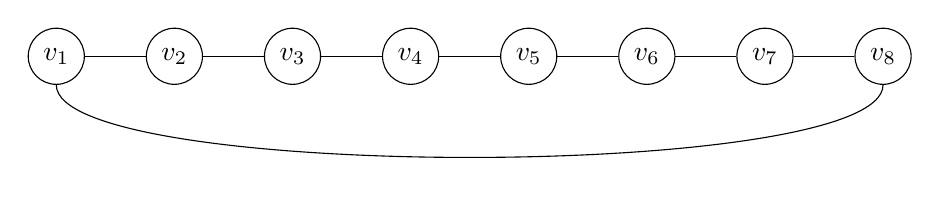
\begin{tikzpicture}[node distance={15mm}, main/.style = {draw, circle}]
		\node[main] (1) {$v_1$};
		\node[main] (2) [right of=1] {$v_2$};
		\node[main] (3) [right of=2] {$v_3$};
		\node[main] (4) [right of=3] {$v_4$};
		\node[main] (5) [right of=4] {$v_5$};
		\node[main] (6) [right of=5] {$v_6$};
		\node[main] (7) [right of=6] {$v_7$};
		\node[main] (8) [right of=7] {$v_8$};
		\draw (1) -- (2);
		\draw (2) -- (3);
		\draw (3) -- (4);
		\draw (4) -- (5);
		\draw (5) -- (6);
		\draw (6) -- (7);
		\draw (7) -- (8);
		\draw (8) to [out=-90,in=-90,looseness=0.3] (1);
	\end{tikzpicture}
	\centering
	\caption{Structure $\mathfrak{G}_1$, consisting of a cycle of length $8$.}
\end{figure}
	\noindent
	While $\mathfrak{G}_2$ is the disjoint structure composed by two cycles of length $4$:
	\begin{figure}[H]
	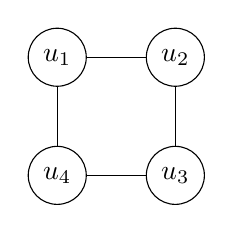
\begin{tikzpicture}[node distance={15mm}, main/.style = {draw, circle}]
		\node[main] (1) {$u_1$};
		\node[main] (2) [right of=1] {$u_2$};
		\node[main] (3) [below of=2] {$u_3$};
		\node[main] (4) [left of=3] {$u_4$};
		\draw (1) -- (2);
		\draw (2) -- (3);
		\draw (3) -- (4);
		\draw (4) -- (1);
	\end{tikzpicture}
	\hspace{3cm}
	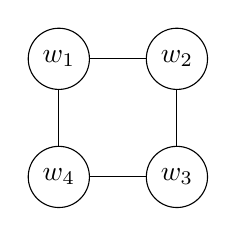
\begin{tikzpicture}[node distance={15mm}, main/.style = {draw, circle}]
		\node[main] (1) {$w_1$};
		\node[main] (2) [right of=1] {$w_2$};
		\node[main] (3) [below of=2] {$w_3$};
		\node[main] (4) [left of=3] {$w_4$};
		\draw (1) -- (2);
		\draw (2) -- (3);
		\draw (3) -- (4);
		\draw (4) -- (1);
	\end{tikzpicture}
	\centering
	\caption{Structure $\mathfrak{G}_2$, consisting of two cycles of length $4$.}
\end{figure}
	
	As we did in the $n = 1$ case, we now simulate a match of the EF-games, analyzing each round individually from both Spoiler's and Discriminator's point of view.
\end{proof}


\begin{exercise}{1.6}
	Consider the following two graphs:
	\begin{enumerate}[\quad{(}1{)}]
		\item $\mathfrak{G}_1$ is a line of length $4n$;
		\item $\mathfrak{G}_2$ consists of a line of length $2n$ and a cycle of length $2n$ (the two components are disjoint).
	\end{enumerate}
	Analyze the EF games on these structures for $n = 1, 2$ and write a sentence of minimal quantifier rank distinguishing the two structures for $n = 1, 2$.
	
	BONUS: Formulate a generalization of your observations and prove that the Acyclicity query is not expressible in the language of graphs over finite graphs, using EF-games.
\end{exercise}
\begin{proof}
Let's discuss every point separately.
\proofpart{$n = 1$.}
In this case, $\mathfrak{G}_1$ is a line of length $4$ (i.e., a graph of containing 5 nodes connected by 4 edges):
\begin{figure}[h]
	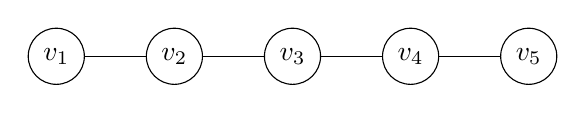
\begin{tikzpicture}[node distance={15mm}, main/.style = {draw, circle}]
		\node[main] (1) {$v_1$};
		\node[main] (2) [right of=1] {$v_2$};
		\node[main] (3) [right of=2] {$v_3$};
		\node[main] (4) [right of=3] {$v_4$};
		\node[main] (5) [right of=4] {$v_5$};
		\draw (1) -- (2);
		\draw (2) -- (3);
		\draw (3) -- (4);
		\draw (4) -- (5);
	\end{tikzpicture}
	\centering
	\caption{Graph $\mathfrak{G}_1$, consisting of a line of length $4$.}
\end{figure}
\noindent
While $\mathfrak{G}_2$ is the disjoint structure composed by a line of length $2$ and a cycle of length $2$:
\begin{figure}[H]
	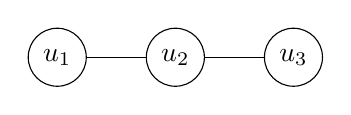
\begin{tikzpicture}[node distance={15mm}, main/.style = {draw, circle}]
		\node[main] (1) {$u_1$};
		\node[main] (2) [right of=1] {$u_2$};
		\node[main] (3) [right of=2] {$u_3$};
		\draw (1) -- (2);
		\draw (2) -- (3);
	\end{tikzpicture}
	\hspace{3cm}
	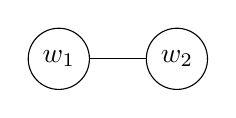
\begin{tikzpicture}[node distance={15mm}, main/.style = {draw, circle}]
		\node[main] (1) {$w_1$};
		\node[main] (2) [right of=1] {$w_2$};
		\draw (1) -- (2);
	\end{tikzpicture}
	\centering
	\caption{Graph $\mathfrak{G}_2$, consisting of a line of length $2$ and cycle of length $2$.}
\end{figure}

Let's now simulate a match of the EF-games, analyzing each round individually from both Spoiler's and Discriminator's point of view. For each round, we will consider all possible scenarios, in order to completely solve the game. We will adopt the usual EF rules:

\begin{itemize}
	\item Spoiler always starts first.
	\item If a player chooses his node from one of the two structures, the other player must necessarily choose his node from the other structure.
	\item Spoiler always tries to win the game in as few moves as possible, while Discriminator always tries to prolong the game as long as possible.
\end{itemize}

\noindent\textbf{Round 1}:

During the first round, each player freely chooses a node from one of the structures. There is no special case to mention.

\noindent\textbf{Round 2}:

During the second round, Spoiler can either select a node connected to the first one, or select a node disconnected from the first one. Either way, Discriminator can respond with a similar move, since both structures contain both connected and disconnected nodes.

\noindent\textbf{Round 3}:

During the third round, there are three possible scenarios. Namely:
\begin{enumerate}
\item Spoiler and Discriminator choose two connected nodes in the first two rounds, in the third round they choose a third node connected to either of the previous two.
\item Spoiler and Discriminator choose two connected nodes in the first two rounds, in the third round they choose a third node not connected to either of the previous two.
\item Spoiler and Discriminator choose two disconnected nodes in the first two rounds, in the third round they choose a third node not connected to either of the previous two.
\end{enumerate}

It's easy to see that all the mentioned scenarios are possible, since both structures contain three connected nodes (e.g., $v_1$, $v_2$, $v_3$ in $\mathfrak{G}_1$, and $u_1$, $u_2$, $u_3$ in $\mathfrak{G}_2$), two connected nodes and a third one disconnected from the first two (e.g., $v_1$, $v_2$, $v_4$ in $\mathfrak{G}_1$, and $u_1$, $u_2$, $e_1$ in $\mathfrak{G}_2$), and three disconnected nodes (e.g., $v_1$, $v_3$, $v_5$ in $\mathfrak{G}_1$, and $u_1$, $u_3$, $w_1$ in $\mathfrak{G}_2$).

Moreover, without loss of generality, we can consider these three as the only possible scenarios. In fact, even if there are still cases that don't follow within those three (e.g., Spoiler and Discriminator choose two disconnected nodes, in the third round they choose a third node connected only to one of the first two), the outcome will still be beneath the cases we described.

\noindent\textbf{Round 4}:

Spoiler chooses three connected nodes in structure $\mathfrak{G}_1$ in the first three rounds, in the fourth round he chooses a fourth node connected to either of the previous three. Therefore, Spoiler wins, since there are no 4 connected nodes in structure $\mathfrak{G}_2$.

\noindent\textbf{Conclusion}:

We saw that Discriminator can win all 3-rounds games on these structures, while he has no winning condition on some of the 4-rounds games. Therefore, $\mathfrak{G}_1$ and $\mathfrak{G}_2$ cannot be distinguished by a sentence of a quantifier-rank $3$ or less (i.e., $\mathfrak{G}_1 \equiv_3 \mathfrak{G}_2$), and there is a sentence of quantifier-rank $4$ with which we can distinguish the two structure (i.e., $\mathfrak{G}_1 \not\equiv_4 \mathfrak{G}_2$).

Specifically, the sentence we empirically used during the game is the one expressing the existence of 4 connected nodes. Formally:

\[
	\exists v_1 \exists v_2 \exists v_3 \exists v_4 (E(v_1, v_2) \land E(v_2, v_3) \land E(v_3, v_4)),
\]
where $E(a, b)$ expresses the existence of an edge between nodes $a$ and $b$.

\proofpart{$n = 2$.}
For $n = 2$, $\mathfrak{G}_1$ is a line of length $8$:
\begin{figure}[H]
	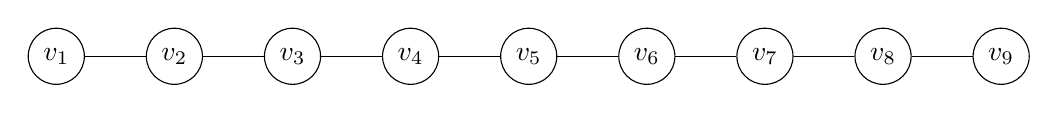
\begin{tikzpicture}[node distance={15mm}, main/.style = {draw, circle}]
		\node[main] (1) {$v_1$};
		\node[main] (2) [right of=1] {$v_2$};
		\node[main] (3) [right of=2] {$v_3$};
		\node[main] (4) [right of=3] {$v_4$};
		\node[main] (5) [right of=4] {$v_5$};
		\node[main] (6) [right of=5] {$v_6$};
		\node[main] (7) [right of=6] {$v_7$};
		\node[main] (8) [right of=7] {$v_8$};
		\node[main] (9) [right of=8] {$v_9$};
		\draw (1) -- (2);
		\draw (2) -- (3);
		\draw (3) -- (4);
		\draw (4) -- (5);
		\draw (5) -- (6);
		\draw (6) -- (7);
		\draw (7) -- (8);
		\draw (8) -- (9);
	\end{tikzpicture}
	\centering
	\caption{Structure $\mathfrak{G}_1$, consisting of a line of length $8$.}
\end{figure}
\noindent
While $\mathfrak{G}_2$ is the disjoint structure composed by a line of length $4$ and a cycle of length $4$:
\begin{figure}[H]
	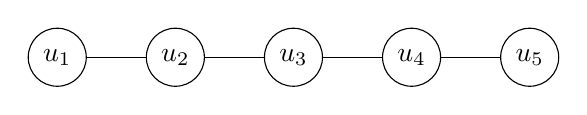
\begin{tikzpicture}[node distance={15mm}, main/.style = {draw, circle}]
		\node[main] (1) {$u_1$};
		\node[main] (2) [right of=1] {$u_2$};
		\node[main] (3) [right of=2] {$u_3$};
		\node[main] (4) [right of=3] {$u_4$};
		\node[main] (5) [right of=4] {$u_5$};
		\draw (1) -- (2);
		\draw (2) -- (3);
		\draw (3) -- (4);
		\draw (4) -- (5);
	\end{tikzpicture}
	\hspace{3cm}
	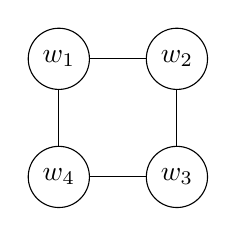
\begin{tikzpicture}[node distance={15mm}, main/.style = {draw, circle}]
		\node[main] (1) {$w_1$};
		\node[main] (2) [right of=1] {$w_2$};
		\node[main] (3) [below of=2] {$w_3$};
		\node[main] (4) [left of=3] {$w_4$};
		\draw (1) -- (2);
		\draw (2) -- (3);
		\draw (3) -- (4);
		\draw (4) -- (1);
	\end{tikzpicture}
	\centering
	\caption{Structure $\mathfrak{G}_2$, consisting of a line of length $4$ and cycle of length $4$.}
\end{figure}

As we did in the $n = 1$ case, we now simulate a match of the EF-games, analyzing each round individually from both Spoiler's and Discriminator's point of view.

\noindent\textbf{Round 1}, \textbf{Round 2} and \textbf{Round 3}:

Equal to the rounds of the $n = 1$ case.

\noindent\textbf{Round 4}:

Spoiler chooses three nodes in the cycle of $\mathfrak{G}_2$ (e.g., $w_1$, $w_2$, $w_3$) during the first three rounds. In the fourth round he chooses the fourth remaining node in the cycle, creating a cycle of length 4. Therefore, Spoiler wins, since there is no cycle of length $4$ in structure $\mathfrak{G}_1$.

\noindent\textbf{Conclusion}:

Similarly to the $n = 1$ case, we saw that Discriminator can win all 3-rounds games on these structures, while he has no winning condition on some of the 3-rounds games. Therefore, $\mathfrak{G}_1$ and $\mathfrak{G}_2$ cannot be distinguished by a sentence of a quantifier-rank $3$ or less (i.e., $\mathfrak{G}_1 \equiv_3 \mathfrak{G}_2$), and there is a sentence of quantifier-rank $4$ with which we can distinguish the two structure (i.e., $\mathfrak{G}_1 \not\equiv_4 \mathfrak{G}_2$).

Specifically, the sentence we empirically used during the game is the one expressing the existence of $4$-cycle. Formally:

\[
\exists v_1 \exists v_2 \exists v_3 \exists v_4 (E(v_1, v_2) \land E(v_2, v_3) \land E(v_3, v_4) \land E(v_4, v_1)),
\]
where $E(a, b)$ expresses the existence of an edge between nodes $a$ and $b$.

\proofpart{Bonus.}

To prove that the acyclicity query is not expressible in the language of graphs over finite graphs, we must show that, for each $k$, it is always possible to choose a pair of graphs, one of which has the property of acyclicity while the other does not, so that these are not distinguishable by a formula of quantifier-rank $k$.
\end{proof}

\end{document}
